%% content.tex
%%

%% ===========================
\chapter{Foundations}
\label{ch:Foundations}
%% ===========================

This chapter provides an introduction to fundamental knowledge that are relevant to this work. We start with the whole SMT system and pre-reordering system first, then followed by the information we used to create the reordering rules including alignment, POS tag, syntax tree. At the end we shows the different rule types, the oracle reordering and how to build lattices for translation. \cite{book} also provide a good introduction to statistical machine translation, including different kinds of theories and methods that are relevant to this work.

%% ===========================
\section{SMT System}
\label{ch:Foundations:sec:SMTSystem}
%% ===========================

%Statistical machine translation (SMT) is a machine translation paradigm where translations are generated on the basis of statistical models whose parameters are derived from the analysis of bilingual text corpora.\cite{wikismt} One typical archit

Statistical machine translation (SMT) is the state of art machine translation paradigm. It uses a typical log-linear model which is composed of a decoder and different statistical models including phrase table, reordering model and language model. All the models are weighted with parameters which are tuned from the development data. Besides development data, training data are used for training the alignment, phrase table and other models. And test data are used for evaluation purpose. The architecture of a SMT system could be illustrated as figure $2.1$.

\begin{figure}[H]
\centering
\newlength{\mylen}
\setlength{\mylen}{0.5cm}

\begin{tikzpicture}[
->,>=stealth', grow=right, level 1/.style={sibling distance=2.4\mylen}, level distance=12\mylen,
node/.style = {align=center, inner sep=0pt, text centered, font=\sffamily, rectangle, rounded corners, draw=black, thick, fill=blue!20, text width=8em, minimum height = 2em, inner sep=5},
nodeimp/.style = {node, fill=red!20},
edge from parent path={(\tikzparentnode.east) -- (\tikzchildnode.west)}
]

\node(A) [node] at (0, 0) {Source Sentences};
\node(C) [node, text width=8em, text height=12em, 
below=1.5\mylen of A] {}
child {node(M) [node, draw=white, fill=white, font=\bfseries] {\LARGE{...}} edge from parent[white]}
child {node(L) [node] {Language Model} edge from parent[white]}
child {node(K) [node] {Reordering Model} edge from parent[white]}
child {node(J) [node] {Phrase Table} edge from parent[white]};

\node(X) [node, draw=blue!20, text width=7em] at (C.center) {Decoder (Global Search)};

\node(D) [node, below=1.5\mylen of C] {Target Sentences};

\draw[->, thick] (A) to (C);
\draw[->, thick] (C) to (D);
\draw[->, thick] (J.west) -- (J-|C.east);
\draw[->, thick] (K.west) -- (K-|C.east);
\draw[->, thick] (L.west) -- (L-|C.east);


%\node(2) [below=1cm of A, node, minimum height = 10 em] at (0\myxa,3\myya) {Decoder};
%\node(3) [node] at (0\myxa,2\myya) {Target Sentences};


%\node(1) [nodeimp] at (3\myxa,4\myya) {Reordering Rules};

%\draw[->] (0) to node [midway, sloped, below] {} node [midway, sloped, above] {} (1);

\end{tikzpicture}
\caption{Architecture of SMT system}
\end{figure}

%% ===========================
\section{Rules Based Pre-Reodering}
\label{ch:Foundations:sec:PreReorderingSystem}
%% ===========================

Our pre-reordering method is based on reordering rules. Reordering rules are rules that tell us how we should reordering the sentences in source language before translating them. In our system, the rules are generated by using the word alignment, part-of-speech (POS) tag and syntax tree, all of which are calculated based on the training data. After we apply the reordering rules to the source sentences, word lattices are generated. The word lattices contains all the reordering possibilities of the source sentences and are further passed to the decoder for translating. The pre-reodering system could be illustrated as figure $2.2$.

\begin{figure}[H]
\centering
\setlength{\mylen}{1cm}

\begin{tikzpicture}[
->,>=stealth', grow=right, level 1/.style={sibling distance=1.3\mylen}, level distance=4\mylen,
node/.style = {align=center, inner sep=0pt, text centered, font=\sffamily, rectangle, rounded corners, draw=black, thick, fill=blue!20, text width=5em, minimum height = 2em, inner sep=5},
nodeimp/.style = {node, fill=red!20}
]


\node(A) [node, text width=8em] at (0, 0) {Sentences in Source Language};
%\node(B) [node, below=\mylen of A] {Reordering};
\node(B) [draw=black, thick, circle, below=\mylen of A] {};
\node(C) [node, text width=8em, below=2\mylen of B] {Decoder (Global Search)};

\draw[-, line width=10pt, white] (C.south west) to (C.south east);
%\node(XX) [below=0.1\mylen of C] {};
%\node(X) [node, draw=white, rounded corners=0, fill=white, maximum height = 0.1em] at (C.south) {};

\node(E) [nodeimp, right=1.4\mylen of B] {Reordering Rules};
\node(EE) [draw=black, thick, circle, right=1.6\mylen of E] {};

\node(F) [nodeimp, above right=0.3*\mylen and 2.85\mylen of E] {Word Alignment};
\node(G) [nodeimp, right=2.85\mylen of E] {POS Tags};
\node(H) [nodeimp, below right=0.3*\mylen and 2.85\mylen of E] {Syntactic Tree};

\node(I) [node, right=\mylen of G] {Training Data};


\draw[->, thick] (A) to (B);
\draw[white] (C) to node[black, midway, sloped, above] {Lattices} (B);
\draw[->, thick] (B) to (C);
\draw[->, thick] (E) to node[midway, above] {Apply} (B);
\draw[->, thick] (EE) to node[midway, above] {Extract} (E);

\node(Saa) [right=0.5\mylen of EE] {};
\node(Sbb) [left=0.5\mylen of I] {};

\coordinate(Sa) at (Saa.base);
\coordinate(Sb) at (Sbb.base);

\draw[->, thick] (Sa) to (EE);
\draw[-, thick] (I) to (Sb);

\draw[-, thick] (F.west) -| (Sa);
\draw[-, thick] (G.west) -| (Sa);
\draw[-, thick] (H.west) -| (Sa);

\draw[->, thick] (Sb) |- (F.east);
\draw[->, thick] (Sb) |- (G.east);
\draw[->, thick] (Sb) |- (H.east);

%\node(2) [below=1cm of A, node, minimum height = 10 em] at (0\myxa,3\myya) {Decoder};
%\node(3) [node] at (0\myxa,2\myya) {Target Sentences};


%\node(1) [nodeimp] at (3\myxa,4\myya) {Reordering Rules};

%\draw[->] (0) to node [midway, sloped, below] {} node [midway, sloped, above] {} (1);

\end{tikzpicture}
\caption{Pre-reordering system}
\end{figure}

A more detailed description of \hyperref[ch:Foundations:sec:Alignment]{word alignment}, \hyperref[ch:Foundations:sec:PosTag]{POS tag}, \hyperref[ch:Foundations:sec:SyntacticTree]{syntax tree},
\hyperref[ch:Foundations:sec:types]{reordering rules} and 
\hyperref[ch:Foundations:sec:Lattices]{word lattices} is also clarified in the following sections.

The \hyperref[ch:ReorderingApproach]{reordering approach} we used for extracting and applying the rules is introduced in the next chapter.

%% ===========================
\section{Word Alignment}
\label{ch:Foundations:sec:Alignment}
%% ===========================

Word alignment indicate the possible alignment between words in the source sentence and words in the target sentence. For example, figure $2.3$ shows an alignment between an English sentence and a Chinese sentence.

\begin{figure}[H]
\centering
\begin{tikzpicture}[
node/.style = {align=center, inner sep=0pt, font=\sffamily, rectangle, draw=white, fill=white, outer sep=0, minimum height=8ex},
]

\node(A1) [node] at (0, 2.2) {$1$ \\ I};
\node(A2) [node, right=1em of A1] {$2$ \\ am};
\node(A3) [node, right=1em of A2] {$3$ \\ a};
\node(A4) [node, right=1em of A3] {$4$ \\ filmmaker};
\node(A5) [node, right=1em of A4] {$5$ \\ .};

\node(B1) [node] at (0, 0) {\cntext{我} \\ $1$};
\node(B2) [node, right=1em of B1] {\cntext{是\vphantom{我}} \\ $2$};
\node(B3) [node, right=1em of B2] {\cntext{一\vphantom{我}} \\ $3$};
\node(B4) [node, right=1em of B3] {\cntext{个\vphantom{我}} \\ $4$};
\node(B5) [node, right=1em of B4] {\cntext{电影\vphantom{我}} \\ $5$};
\node(B6) [node, right=1em of B5] {\cntext{制片人\vphantom{我}} \\ $6$};
\node(B7) [node, right=1em of B6] {\cntext{。\vphantom{我}} \\ $7$};

\draw[-, thick] (A1.south) -- (B1.north);
\draw[-, thick] (A2.south) -- (B1.north);
\draw[-, thick] (A2.south) -- (B2.north);
\draw[-, thick] (A3.south) -- (B3.north);
\draw[-, thick] (A3.south) -- (B4.north);
\draw[-, thick] (A4.south) -- (B5.north);
\draw[-, thick] (A4.south) -- (B6.north);
\draw[-, thick] (A5.south) -- (B7.north);

\end{tikzpicture}
\caption{Example of word alignment}
\end{figure}
%? better example with crossing alignment?
Or it may be simply presented as index pairs.
\begin{center}
\verb|7-1 8-1 8-2 9-3 9-4 1-5 1-6 2-6 5-6 3-7 4-8 4-9 10-10|
\end{center}

In the figure, the words that are aligned through lines in two languages have related meaning. We can see how the words are reordered from the figure. For exmaple, the noun clause ``Clinton's presidency'' is completely moved forward to the front of the sentence.

\phantomsection\label{alignedrange}
It is noteworthy that the alignment is not always a one-to-one match. In the example, the word ``of'' is not aligned at all and the word ``months'' is aligned to two word ``\cntext{个}'' and ``\cntext{月}'' in Chinese. We can define the aligned range as the range from the first word a certain word is aligned to to the last word it is aligned to. For example, the aligned range of word ``there'' is $[5,6]$. The \textbf{aligned range} can be coincided, such as the $6$th word ``\cntext{剩下}'' in Chinese is also aligned to ``are'' and ``left'' at the same time besides ``there''. The coincidence sometimes makes the detection of rules more difficult, because the word order is not clear any more.

The word alignment could be trained with the GIZA++ tool by using Expectation Maximization (EM) algorithm. From the word alignment of training data we can see the patterns how the words are reordered before and after translation. Therefore, we could extract these reordering rules and apply them on the text, which is to be translated.

%% ===========================
\section{Part-of-Speech Tag}

Part-of-speech (POS) tags are markups of words in the text, which corresponds their linguistic role in the text. Depends on the definition of the roles, the set of POS tags could be different. Besides, different languages may have different POS tag set, since they may have different linguistic features, which are relevant to translation.
\begin{figure}[H]
\centering
\begin{tikzpicture}[
node/.style = {align=center, inner sep=0pt, font=\sffamily, rectangle, draw=white, fill=white, outer sep=0, text height=5ex},
]

\node(A) [node] {The \\ DT};
\node(B) [node, right=1ex of A] {domestic \\ JJ};
\node(C) [node, right=1ex of B] {consumption \\ NN};
\node(D) [node, right=1ex of C] {market \\ NN};
\node(E) [node, right=1ex of D] {for \\ IN};
\node(F) [node, right=1ex of E] {animal \\ NN};
\node(G) [node, right=1ex of F] {products \\ NNS};
\node(H) [node, right=1ex of G] {is \\ VBZ};
\node(I) [node, right=1ex of H] {very \\ RB};
\node(J) [node, right=1ex of I] {great \\ JJ};
\node(K) [node, right=1ex of J] {. \\ SENT};



\end{tikzpicture}
\caption{Example of POS tags}
\end{figure}
Figure $2.4$ shows an tagged English sentence. 

Tagset? English \& Chinese how to tag?


\label{ch:Foundations:sec:PosTag}
%% ===========================

%% ===========================
\section{syntax tree}
\label{ch:Foundations:sec:SyntacticTree}
%% ===========================

The syntax tree shows the syntactic structure of a sentence and can be very useful for word reordering. A syntax tree contains two kinds of nodes: the leaves and the internal nodes. Each leaf presents a word in the sentence, and is annotated with the POS tag. And each internal node presents a constituents, which is also annotated to indicate its category or syntactic role. In the Penn treebank \citep{penn}, for example, the annotation ``NP'' means noun phrase and the annotation ``S'' means simple declarative clause. Figure $2.5$ is an example of a syntax tree.

\begin{figure}[H]
\centering
\begin{tikzpicture}[
-,>=stealth',
level/.style={sibling distance = 2cm, level distance = 1.8cm},
%level 1/.style={sibling distance=8cm},
%level 2/.style={sibling distance=4cm}, 
%level 3/.style={sibling distance=4cm}, 
treenode/.style = {align=center, inner sep=0pt, text centered, font=\sffamily},
arn_n/.style = {treenode, rectangle, rounded corners, draw=black, thick, fill=blue!20, minimum width=4em, minimum height = 2em},
arn_x/.style = {arn_n, fill=red!20, minimum height=3em},
edge from parent fork down
]
\node [arn_n] {S}
child[sibling distance = 6cm]{ node [arn_n] {NP}
child{ node [arn_x] {NN\\ math}}
child{ node [arn_x] {CC\\ and}}
child{ node [arn_x] {NN\\ biology}}
child{ node [arn_x] {NNS\\ exams}}}
child{ node [arn_n] {VP}
child{ node [arn_x] {MD\\ will}}
child{ node [arn_n] {VP}
child{ node [arn_x] {VB\\ be}}
child{ node [arn_n] {PP}
child{ node [arn_x] {IN\\ on}}
child{ node [arn_n] {NP}
child{ node [arn_x] {DT\\ the}}
child{ node [arn_x] {JJ\\ 27th}}}}}}
child[sibling distance = 4.2cm]{ node [arn_x] {.\\ .}};
\end{tikzpicture}
\caption{Example of a parse tree}
\end{figure}

We can see the syntactic structure of the sentence from the syntax tree very clear. In this example, The words ``math and biology exams'' make up a noun clause, which plays the roll of subject. The predicate has a nested structure of verb clause, because it's compound with the modal verb ``will'' and the word ``be''. And ``on the 27th'' is a preposition clause in the verb clause, which is again composed of a preposition ``in'' and a noun clause ``the 27th''.

%%% ===========================
%\section{Dependency Tree}
%\label{ch:Foundations:sec:DependencyTree}
%%% ===========================

%% ===========================
\section{Reordering Rules}
\label{ch:Foundations:sec:types}
%% ===========================
%Short rules was introduced by \cite{short}.
%\subsection{Short Rules}
%\subsection{Long Rules}
%\subsection{Tree Rules}

Based on \cite{short}, \cite{long}, \cite{tree} and \cite{combine}, we introduce the different rule types, rule combination, how to decide if rules can be extracted as well as how to calculate the probability to apply the rules.

\subsection{Short Rules}

Short rules are extracted based on the sequences of adjacent words or their POS tags in the sentence to translate. Sequences of adjacent words or tags are observed, rules are then extracted if the same reordering patterns appear frequently. Following are some examples:
$$\verb|after the accident -> the accident after (0.5)|$$
$$\verb|WRB MD DT -> DT WRB DT (0.3)|$$
The first rule in this example shows, if a the word sequence ``after the accident'' ever appears in the text, it should be reordered to ``the accident after'' with a probability $0.5$, so will the word order be more consistent with the translation. The second rule shows, if the word sequence of a wh-adverb (when, where, why, etc.), a modal verb (MD) and a determiner (DT) appears, the determiner should be moved before the wh-adverb with a probablity of $0.3$.

In addition, Short rules also have some different varieties \citep{short}:
\begin{itemize}
\setlength{\itemsep}{0cm}%
\setlength{\parskip}{0cm}%
\item \textbf{Tag sequence:} rules are extracted based on adjacent tag sequence
\item \textbf{Word sequence:} rules are extracted based on adjacent word sequence
\item \textbf{Context of one or two tags before and/or after the tag sequence}
\item \textbf{Context of one or two words before and/or after the tag sequence}
\end{itemize}

\subsection{Long Rules}

Long rules are specially designed to help the long distance word reordering for translation between English and German. The rules are based on POS tags of the text, and an example is as following:
$$\verb|NN X MD VHP -> X MD NN VHP (0.14)|$$

The ``X'' in the example is an placeholder, which can replace one or more words. ``VHP'' is the right context, which is sometimes helpful to define the reordering boundary. ``NN'' means noun, ``MD'' means modal verb and ``VHP'' is the word ``have''. In this example, the tag sequence ``NN X MD VHP'' will be reordered as ``X MD NN VHP'' with a likelihood of $0.1429$.

Rules are extracted by first finding the location of the reordering rule and then putting the placeholder. Depends on the location, where the placeholder is put, and how much the placeholder replace,  the long rules also have some varieties:
\begin{itemize}
\setlength{\itemsep}{0cm}%
\setlength{\parskip}{0cm}%
\item \textbf{Left/right rules:} depends on if the placeholder is put on the left part or right part
\item \textbf{All/part replacement:} depends on if all the words in a part is replaced by the placeholder
\end{itemize}

\subsection{Tree Rules}
\label{treerules}

While short rules and long rules are based on the flat structure of the sentence, tree rules reorders the sentence by using information from the sentence's syntactic structure. The syntax tree and alignment of the training corpus are used to train the rules. The tree rules reorder the words both on the word level and on the constituent level. Following is an example:
$$\verb|NP ( ADJP JJ NN ) -> JJ NN ADJP (0.06)|$$
The parenthesis in the example represents the hierarchies in the syntax tree. The left side of the rule corresponds a tree with root labeled with ``NP'' and three children, each labeled with ``JJ'', ``NN'' and ``ADJP''. When this structure appears as a subtree in the syntax tree of the sentence to translate, the order of its subtrees should be changed. The change is illustrated in figure $f$.

\begin{figure}[H]
\centering
\begin{tikzpicture}[
-,>=stealth',
level/.style={sibling distance = 1.8cm, level distance = 1.8cm},
%level 1/.style={sibling distance=8cm},
%level 2/.style={sibling distance=4cm}, 
%level 3/.style={sibling distance=4cm}, 
treenode/.style = {align=center, minimum width=3.8em, minimum height = 2em, inner sep=0pt, text centered, font=\sffamily},
arn_n/.style = {treenode, rectangle, rounded corners, draw=black,  fill=blue!20},
arn_x/.style = {arn_n, fill=red!20, font=\itshape, rounded corners=0},
edge from parent fork down
]
\node (A) [arn_n] {NP}
child{ node [arn_x] {ADJP}}
child{ node [arn_x] {JJ}}
child{ node (X) [arn_x] {NN}};



\node (B) [arn_n, right = 5.4cm of A] {NP}
child{ node (Y) [arn_x] {JJ}}
child{ node [arn_x] {NN}}
child{ node [arn_x] {ADJP}};

\node (XX) [below right=0.2cm and 2cm of A] {};
\node (YY) [below left= 0.2cm and 2cm of B] {};


%\draw[-,double distance=2pt] (XX) to (YY);
%\draw[open triangle 60, thick] (XX) to (YY);
\draw[draw=none] (XX) to node[draw, midway, single arrow] {\Hstrut\Hstrut\Hstrut} (YY);
\end{tikzpicture}


\caption{Change subtree order based on tree rules}
\end{figure}

Tree rules also have some different varieties:
\begin{itemize}
\setlength{\itemsep}{0cm}%
\setlength{\parskip}{0cm}%
\item \textbf{Partial Rules:} the relatively flat syntactic structure of languages like German may make the rule extraction difficult, because the extraction requires that the whole subtree including all its children is matched. In order to extract more useful information for reordering, rules are also extracted from any partial child sequence in a constituent.
\item \textbf{Recursive rule application:} the rules may be applied recursively to already reordered sentence. And all paths of the reorderings are added to the lattice.
\end{itemize}


\subsection{Rule Extraction and Application}
\label{general}

Rules are extracted by scanning all the training data and detecting the word order change. A valid word order change that can count for reordering rule needs to fulfill the two criteria in general:
\begin{itemize}
\setlength{\itemsep}{0cm}%
\setlength{\parskip}{0cm}%
\item \textbf{Order change exists:} otherwise, there's no need for reordering rules.
\item \textbf{No \hyperref[alignedrange]{aligned ranges} coincidence:} the coincidence makes it hard to decide the new word orders in target language.
\end{itemize}

Rules are not always extracted upon discovering of word change. In order to avoid too excessively concrete rules which don't apply well in general, we extract reordering rules only when the same reordering pattern appears more than a certain threshold. Thus it won't lead to overfitting.

The associated probabilities of reordering rules is the frequency how often the sequence in the rules are reordered in the same manner. For example, if the sequence ``after the accident'' appears many times in the training data, and half of the time, it's reordered as ``the accident after'', then the probability of the reordering rule is calculated as $50\%$.

Rules are applied by scanning the text to be translated. When there's a sequence coincides the left side of the reordering rules, rules will be applied, and a path in the \hyperref[ch:Foundations:sec:Lattices]{word lattice} representing the reordered word will be added.

\subsection{Rule Combination}

In order to further explore the probability of improvement, we combine different rules for reordering in our experiment. This is done by training the different types of rules separately and applying them on the monotone path of the sentence independently. They result different paths in the lattice.



%% ===========================
\section{Oracle Reordering}
\label{ch:Foundations:sec:oracle}
%% ===========================



%% ===========================
\section{Word Lattice}
\label{ch:Foundations:sec:Lattices}
\label{latticecreation}
%% ===========================
A word lattice could be presented with a directed acyclic graph. The graph contains nodes and transitions, with each transition labeled with a word and a probability. The outgoing transitions from a node indicate different options, which words could come after this point. The annotation on the transition indicate the word that could come, together with the probability of this option. The word lattice groups different word reorderings of the same English sentence together, with each reordering corresponding a path from the beginning node to the end node. 

Word lattice for reordered word sequences is build gradually while applying the reordering rules on the sentence. It starts with a monotone path presenting the sentence to translated. Every time when a rule is applied and part of the sentence is reordered. We add a parallel path to the corresponding part of the initial monotone path. The parallel path is labeled with reordered words on its transitions. The probability of this new reordering is subtracted from the first transition after the splitting point on monotone path, and assigned to the first transition of the new path. All the other transitions on the new path that follow have a probability of $1$.

%? graph for building?

Paths with very low probability are removed, in order to save space for storing the lattice and reduce decoding time later, without compromising to much translation quality. %?In our system, we remove all the paths that have a probability lower than $0.1$.

An example of a word lattice is showed in figure $2.6$. If the probability of a transition is $1$, it's left out in the example to keep the graph clear.


\begin{landscape}
\begin{figure}
\centering
\begin{tikzpicture}[
nod_s/.style = {align=center, inner sep=2pt, text centered, font=\sffamily, circle, draw},
nod_m/.style = {nod_s, thick},
edge_ls/.style = {},
edge_lm/.style = {edge_ls, thick},
edge_ts/.style = {font=\tiny},
edge_tm/.style = {edge_ts},
]

\newlength{\myx}
\setlength{\myx}{1.3cm}
\newlength{\myy}
\setlength{\myy}{1.2cm}

\node(0) [nod_m] at (0\myx,0\myy) {};
\node(1) [nod_m] at (1\myx,0\myy) {};
\node(2) [nod_s] at (1\myx,1\myy) {};
\node(3) [nod_m] at (2\myx,0\myy) {};
\node(4) [nod_s] at (2\myx,1\myy) {};
\node(5) [nod_m] at (3\myx,0\myy) {};
\node(6) [nod_m] at (4\myx,0\myy) {};
\node(7) [nod_m] at (5\myx,0\myy) {};
\node(8) [nod_s] at (5\myx,1\myy) {};
\node(9) [nod_m] at (6\myx,0\myy) {};
\node(10) [nod_m] at (7\myx,0\myy) {};
\node(11) [nod_s] at (7\myx,1\myy) {};
\node(12) [nod_m] at (8\myx,0\myy) {};
\node(13) [nod_m] at (9\myx,0\myy) {};
\node(14) [nod_s] at (9\myx,5\myy) {};
\node(15) [nod_s] at (9\myx,6\myy) {};
\node(16) [nod_s] at (9\myx,7\myy) {};
\node(17) [nod_m] at (10\myx,0\myy) {};
\node(18) [nod_s] at (10\myx,5\myy) {};
\node(19) [nod_s] at (10\myx,6\myy) {};
\node(20) [nod_s] at (10\myx,7\myy) {};
\node(21) [nod_m] at (11\myx,0\myy) {};
\node(22) [nod_s] at (11\myx,1\myy) {};
\node(23) [nod_s] at (11\myx,4\myy) {};
\node(24) [nod_s] at (11\myx,5\myy) {};
\node(25) [nod_s] at (11\myx,6\myy) {};
\node(26) [nod_s] at (11\myx,7\myy) {};
\node(27) [nod_m] at (12\myx,0\myy) {};
\node(28) [nod_s] at (12\myx,4\myy) {};
\node(29) [nod_s] at (12\myx,5\myy) {};
\node(30) [nod_s] at (12\myx,6\myy) {};
\node(31) [nod_s] at (12\myx,7\myy) {};
\node(32) [nod_m] at (13\myx,0\myy) {};
\node(33) [nod_s] at (13\myx,3\myy) {};
\node(34) [nod_s] at (13\myx,4\myy) {};
\node(35) [nod_s] at (13\myx,5\myy) {};
\node(36) [nod_s] at (13\myx,6\myy) {};
\node(37) [nod_s] at (13\myx,7\myy) {};
\node(38) [nod_m] at (14\myx,0\myy) {};
\node(39) [nod_s] at (14\myx,2\myy) {};
\node(40) [nod_s] at (14\myx,3\myy) {};
\node(41) [nod_s] at (14\myx,4\myy) {};
\node(42) [nod_s] at (14\myx,5\myy) {};
\node(43) [nod_s] at (14\myx,6\myy) {};
\node(44) [nod_s] at (14\myx,7\myy) {};
\node(45) [nod_m] at (15\myx,0\myy) {};
\node(46) [nod_s] at (15\myx,1\myy) {};
\node(47) [nod_s] at (15\myx,2\myy) {};
\node(48) [nod_s] at (15\myx,3\myy) {};
\node(49) [nod_s] at (15\myx,4\myy) {};
\node(50) [nod_s] at (15\myx,5\myy) {};
\node(51) [nod_s] at (15\myx,6\myy) {};
\node(52) [nod_s] at (15\myx,7\myy) {};
\node(53) [nod_m] at (16\myx,0\myy) {};
\node(54) [nod_m] at (17\myx,0\myy) {};

\draw[->,edge_lm] (0) to node [midway, sloped, below, edge_tm] {satisfying} node [midway, sloped, above, edge_tm] {0.8688} (1);
\draw[->,edge_ls] (0) to [bend left] node [midway, sloped, above, edge_ts] {personal} node [midway, sloped, below, edge_ts] {0.1312} (2);
\draw[->,edge_lm] (1) to node [midway, sloped, below, edge_tm] {personal} (3);
\draw[->,edge_ls] (2) to node [midway, sloped, above, edge_ts] {interests} (4);
\draw[->,edge_lm] (3) to node [midway, sloped, below, edge_tm] {interests} (5);
\draw[->,edge_ls] (4) to [bend left] node [midway, sloped, above, edge_ts] {satisfying} (5);
\draw[->,edge_lm] (5) to node [midway, sloped, below, edge_tm] {and} (6);
\draw[->,edge_lm] (6) to node [midway, sloped, below, edge_tm] {expanding} node [midway, sloped, above, edge_tm] {0.8688} (7);
\draw[->,edge_ls] (6) to [bend left] node [midway, sloped, above, edge_ts] {knowledge} node [midway, sloped, below, edge_ts] {0.1312} (8);
\draw[->,edge_lm] (7) to node [midway, sloped, below, edge_tm] {knowledge} (9);
\draw[->,edge_ls] (8) to [bend left] node [midway, sloped, above, edge_ts] {expanding} (9);
\draw[->,edge_lm] (9) to node [midway, sloped, below, edge_tm] {are} node [midway, sloped, above, edge_tm] {0.3049} (10);
\draw[->,edge_ls] (9) to [bend left] node [midway, sloped, above, edge_ts] {also} node [midway, sloped, below, edge_ts] {0.6951} (11);
\draw[->,edge_lm] (10) to node [midway, sloped, below, edge_tm] {also} (12);
\draw[->,edge_ls] (11) to [bend left] node [midway, sloped, above, near start, edge_ts] {are} (12);
\draw[->,edge_lm] (12) to node [midway, sloped, below, edge_tm] {major} node [midway, sloped, above, edge_tm] {0.4046} (13);
\draw[->,edge_ls] (12) to [bend left] node [midway, sloped, above, very near end, edge_ts] {why} node [midway, sloped, below, very near end, edge_ts] {0.3406} (14);
\draw[->,edge_ls] (12) to [bend left] node [midway, sloped, above, very near end, edge_ts] {work} node [midway, sloped, below, very near end, edge_ts] {0.1226} (15);
\draw[->,edge_ls] (12) to [bend left] node [midway, sloped, above, very near end, edge_ts] {work} node [midway, sloped, below, very near end, edge_ts] {0.1321} (16);
\draw[->,edge_lm] (13) to node [midway, sloped, below, edge_tm] {reasons} (17);
\draw[->,edge_ls] (14) to node [midway, sloped, above, edge_ts] {hourly} (18);
\draw[->,edge_ls] (15) to node [midway, sloped, above, edge_ts] {appeals} (19);
\draw[->,edge_ls] (16) to node [midway, sloped, above, edge_ts] {appeals} (20);
\draw[->,edge_lm] (17) to node [midway, sloped, below, edge_tm] {why} node [midway, sloped, above, edge_tm] {0.3641} (21);
\draw[->,edge_ls] (17) to [bend left] node [midway, sloped, above, edge_ts] {hourly} node [midway, sloped, below, edge_ts] {0.1813} (22);
\draw[->,edge_ls] (17) to [bend left] node [midway, sloped, above,  edge_ts] {work} node [midway, sloped, below, edge_ts] {0.4545} (23);
\draw[->,edge_ls] (18) to node [midway, sloped, above, edge_ts] {work} (24);
\draw[->,edge_ls] (19) to node [midway, sloped, above, edge_ts] {to} (25);
\draw[->,edge_ls] (20) to node [midway, sloped, above, edge_ts] {to} (26);
\draw[->,edge_lm] (21) to node [midway, sloped, below, edge_tm] {hourly} (27);
\draw[->,edge_ls] (22) to [bend left] node [midway, sloped, above, edge_ts] {why} (27);
\draw[->,edge_ls] (23) to node [midway, sloped, above, edge_ts] {appeals} (28);
\draw[->,edge_ls] (24) to node [midway, sloped, above, edge_ts] {appeals} (29);
\draw[->,edge_ls] (25) to node [midway, sloped, above, edge_ts] {people} (30);
\draw[->,edge_ls] (26) to node [midway, sloped, above, edge_ts] {people} (31);
\draw[->,edge_lm] (27) to node [midway, sloped, below, edge_tm] {work} node [midway, sloped, above, edge_tm] {0.5677} (32);
\draw[->,edge_ls] (27) to [bend left] node [midway, sloped, above, edge_ts] {to} node [midway, sloped, below, edge_ts] {0.4323} (33);
\draw[->,edge_ls] (28) to node [midway, sloped, above, edge_ts] {to} (34);
\draw[->,edge_ls] (29) to node [midway, sloped, above, edge_ts] {to} (35);
\draw[->,edge_ls] (30) to node [midway, sloped, above, edge_ts] {major} (36);
\draw[->,edge_ls] (31) to node [midway, sloped, above, edge_ts] {why} (37);
\draw[->,edge_lm] (32) to node [midway, sloped, below, edge_tm] {appeals} node [midway, sloped, above, edge_tm] {0.8004} (38);
\draw[->,edge_ls] (32) to [bend left] node [midway, sloped, above, edge_ts] {to} node [midway, sloped, below, edge_ts] {0.1996} (39);
\draw[->,edge_ls] (33) to node [midway, sloped, above, edge_ts] {people} (40);
\draw[->,edge_ls] (34) to node [midway, sloped, above, edge_ts] {people} (41);
\draw[->,edge_ls] (35) to node [midway, sloped, above, edge_ts] {people} (42);
\draw[->,edge_ls] (36) to node [midway, sloped, above, edge_ts] {reasons} (43);
\draw[->,edge_ls] (37) to node [midway, sloped, above, edge_ts] {hourly} (44);
\draw[->,edge_lm] (38) to node [midway, sloped, below, edge_tm] {to} node [midway, sloped, above, edge_tm] {0.8966} (45);
\draw[->,edge_ls] (38) to [bend left] node [midway, sloped, above, edge_ts] {people} node [midway, sloped, below, edge_ts] {0.1034} (46);
\draw[->,edge_ls] (39) to node [midway, sloped, above, edge_ts] {people} (47);
\draw[->,edge_ls] (40) to node [midway, sloped, above, edge_ts] {work} (48);
\draw[->,edge_ls] (41) to node [midway, sloped, above, edge_ts] {why} (49);
\draw[->,edge_ls] (42) to node [midway, sloped, above, edge_ts] {major} (50);
\draw[->,edge_ls] (43) to node [midway, sloped, above, edge_ts] {why} (51);
\draw[->,edge_ls] (44) to node [midway, sloped, above, edge_ts] {major} (52);
\draw[->,edge_lm] (45) to node [midway, sloped, below, edge_tm] {people} (53);
\draw[->,edge_ls] (46) to [bend left] node [midway, sloped, above,  near start, edge_ts] {to} (53);
\draw[->,edge_ls] (47) to [bend left] node [midway, sloped, above, very near start, edge_ts] {appeals} (53);
\draw[->,edge_ls] (48) to [bend left] node [midway, sloped, above, very near start, edge_ts] {appeals} (53);
\draw[->,edge_ls] (49) to [bend left] node [midway, sloped, above, very near start, edge_ts] {hourly} (53);
\draw[->,edge_ls] (50) to [bend left] node [midway, sloped, above, very near start, edge_ts] {reasons} (53);
\draw[->,edge_ls] (51) to [bend left] node [midway, sloped, above, very near start, edge_ts] {hourly} (53);
\draw[->,edge_ls] (52) to [bend left] node [midway, sloped, above, very near start, edge_ts] {reasons} (53);
\draw[->,edge_lm] (53) to node [midway, sloped, below, edge_tm] {\vphantom{people}.} (54);

\end{tikzpicture}
\caption{Example of a word lattice}
\end{figure}
\end{landscape}

\section{BLEU Score}
\label{ch:Foundations:sec:bleu}
BLEU is the de facto standard in machine translation\cite{metrics}. We use BLEU score to evaluate the SMT system throughout this paper.


\section{Summary}

%% ===========================
\chapter{Reordering Approach}
\label{ch:ReorderingApproach}
%% ===========================

%% ===========================
\section{Reordering Problem in Chinese Translation}
\label{ch:ReorderingApproach:sec:Problem}
%% ===========================

English and Chinese belong to different language groups. As Chinese belong to the Sino-Tibet language group, while English belong to the Indo-Germanic language group. And they have also developed separately for a long time. Because of their different origins and development, they've becoming two very different languages.

Unlike the most languages in the Indo-Germanic language group, which are more close to English than Chinese, Chinese has some properties those languages don't have, such as Characters as fundamental element instead of letters, the tones, no word separation, the usage of measure words,much more simple inflections and conjugations, which raises further problem for machine translation.

Even the word order between English and Chinese is more distinct. For one, the words in Chinese have generally different origins as those in English, which leads to different vocabulary and sometimes it's very hard to found corresponding words in the other language. For example, Chinese has a lot of different prepositions and adverbs, which have very distinct usage as those in English. Also the continuous writing of Chinese without space makes this problem more severe, since word boundaries are not always so clear in Chinese. Text needs to be segmented before translation, and a word segmentation program decide how to separate the words and the result is not always ideal.

For the other, 

And sometimes, a long English sentence with clauses is more suitable to be translated into two of more Chinese sentences. Through analyzing the data we have, we've found several major word order differences between English and Chinese, which leads to low translation quality and should be changed. 

%? examples of different kinds for word order differences

\cite{syntactic} also systematic analyzing about Chinese syntactic reordering. Through our analyzing / research, examples below, worth noticing / improving

``Quote'':


Mandarin Chinese sentence structure is quite different than English or other European languages. Since the word order doesn't match, sentences which are translated word-for-word to Mandarin will be difficult to understand. You must learn to think in Mandarin Chinese when speaking the language. 

There're plenty of literatures discussing the sentence strucutes of chinese cite.. please.

\paragraph{Preposition phrases}

\paragraph{relation clauses}

\paragraph{Adverbials}
An adverbial can be an adverb, an adverbial phrase or an adverbial clause that modifies the verb or the whole sentence. The position of adverbials is a complicated topic. In general, the location of adverbials in a sentence are very flexible. They can be located in different position of a sentence both in English and Chinese, such as beginning, middle or end of a sentence, before or after the verb. The location varies and it often depends on the situation. When comparing English and Chinese word order, the location of adverbials in one language doesn't automatically implies the same location in the other. Typical examples are adverbials of time, location and frequency. It's often put after the verb in English, but before the verb in Chinese. 
\begin{figure}[H]
\centering
%\begin{tikzpicture}[
node/.style = {align=center, inner sep=2pt, font=\sffamily, rectangle, draw=none, fill=white, outer sep=0, minimum height=8ex},
]
%Cloning will happen in five to 10 years .
%克隆 将 在 未来 5 到 10 年 内 发生 。
%1-1 2-2 4-3 3-4 5-5 6-6 7-7 8-8 8-9 3-10 9-11

\begin{scope}[start chain=1 going below,start chain=2 going right]
\node[on chain=1] (A) {A};
\node[on chain=1] (C) {C};
\node[on chain=1] (D) {D};
\node[on chain=1] (G) {G};
\node[on chain=1] (H) {H};
\chainin (A);
\node[on chain=2,] (B) {B};
\node[continue chain=going below,on chain=2] (E) {E};
\node[on chain=2] (F) {F};
\end{scope}



%\node(A1) [node] at (0, 5) {$1$ \\ There};
%\node(A2) [node, right=1em of A1] {$2$ \\ are};
%\node(A3) [node, right=1em of A2] {$3$ \\ four};
%\node(A4) [node, right=1em of A3] {$4$ \\ months};
%\node(A5) [node, right=1em of A4] {$5$ \\ left};
%\node(A6) [node, right=1em of A5] {$6$ \\ of};
%\node(A7) [node, right=1em of A6] {$7$ \\ Clinton};
%\node(A8) [node, right=1em of A7] {$8$ \\ 's};
%\node(A9) [node, right=1em of A8] {$9$ \\ presidency};
%\node(A10) [node, right=1em of A9] {$10$ \\ .};
%
%\node(B1) [node] at (0, 0) {\cntext{克林顿} \\ $1$};
%\node(B2) [node, right=1.53em of B1] {\cntext{的\vphantom{我}} \\ $2$};
%\node(B3) [node, right=1.53em of B2] {\cntext{总统\vphantom{我}} \\ $3$};
%\node(B4) [node, right=1.53em of B3] {\cntext{任期\vphantom{我}} \\ $4$};
%\node(B5) [node, right=1.53em of B4] {\cntext{还\vphantom{我}} \\ $5$};
%\node(B6) [node, right=1.53em of B5] {\cntext{剩下\vphantom{我}} \\ $6$};
%\node(B7) [node, right=1.53em of B6] {\cntext{四\vphantom{我}} \\ $7$};
%\node(B8) [node, right=1.53em of B7] {\cntext{个\vphantom{我}} \\ $8$};
%\node(B9) [node, right=1.53em of B8] {\cntext{月\vphantom{我}} \\ $9$};
%\node(B10) [node, right=1.53em of B9] {\cntext{。\vphantom{我}} \\ $10$};
%
%\draw[dashed, thick] (A7.south) -- (B1.north);
%\draw[dashed, thick] (A8.south) -- (B1.north);
%\draw[dashed, thick] (A8.south) -- (B2.north);
%\draw[dashed, thick] (A9.south) -- (B3.north);
%\draw[dashed, thick] (A9.south) -- (B4.north);
%\draw[dashed, thick] (A1.south) -- (B5.north);
%\draw[dashed, thick] (A1.south) -- (B6.north);
%\draw[dashed, thick] (A2.south) -- (B6.north);
%\draw[dashed, thick] (A5.south) -- (B6.north);
%\draw[dashed, thick] (A3.south) -- (B7.north);
%\draw[dashed, thick] (A4.south) -- (B8.north);
%\draw[dashed, thick] (A4.south) -- (B9.north);
%\draw[dashed, thick] (A10.south) -- (B10.north);

\end{tikzpicture}

\caption{Position change of an adverbial of time}
\end{figure}


\paragraph{questions}

\paragraph{There be ...}
%?correct compound subjects: or & there be...
%% ===========================
\section{Motivation of Reordering on Multiple Syntactic Levels}
\label{ch:ReorderingApproach:sec:Motivation}
%% ===========================


%? long distance position change, unstructural position change.

\subsection{Long Distance Word Reordering}

efficient than hier

use tree and alignment only

\subsection{Unstructured Word Reordering}

Because English and Chinese have different word orders and there're also some special cases of sentence patterns, the word reordering can be complicated and unsystematically. Sometimes it involves word position changes on multiple syntactic levels. We can see this problem from the examples in figure $3.1$. In the figure, the syntactic structure and alignment of the parallel text are presented in a intuitive way.

\begin{figure}[H]
\centering
\subfigure {
\input{unstructured.tikz}
}
\subfigure {
\begin{tikzpicture}[scale=0.5,
-,>=stealth',
level/.style={sibling distance = 3cm, level distance = 1.8cm},
level 1/.style={sibling distance=6cm},
level 2/.style={sibling distance=4cm}, 
%level 3/.style={sibling distance=4cm}, 
treenode/.style = {scale=0.5, align=center, inner sep=0.5em, text centered, font=\sffamily},
arn_n/.style = {treenode, rectangle, rounded corners=0.75mm, draw=black,  fill=blue!20, minimum width=4em, minimum height = 2em},
arn_x/.style = {arn_n, fill=blue!20, minimum height=3em, rounded corners=0},
edge from parent fork down
]
\node [arn_n, fill=red!20, font=\itshape] {S}
child{ node [arn_n, fill=red!20, font=\itshape] {NP}
child{ node [arn_n, fill=red!40, font=\itshape] {NP}
child{ node [arn_n] {QP}
child{ node [arn_x](A) {CD\\ four}}
child{ node [arn_x](B) {CD\\ million}}}}
child{ node [arn_n, fill=red!40, font=\itshape] {PP}
child{ node [arn_x](C) {IN\\ of}}
child{ node [arn_n] {NP}
child{ node [arn_x](D) {DT\\ these}}
child{ node [arn_x](E) {NNS\\ babies}}}}}
child{ node [arn_n, fill=red!20, font=\itshape] {VP}
child{ node [arn_x, fill=red!40, font=\itshape](F) {VBP\\ die}}
child{ node [arn_n, fill=red!40, font=\itshape] {ADVP}
child{ node [arn_x](G) {RB\\ annually}}}}
child [sibling distance = 3.5cm]{ node [arn_x, fill=red!40, font=\itshape](H) {.\\ .}};

\node [below right=5.5cm and 0.2cm of H.south west, scale=0.75](Q) {\cntext{\vphantom{存}。}};
\node [left=0.09cm of Q, scale=0.75](P) {\cntext{存活}};
\node [left=0.09cm of P, scale=0.75](O) {\cntext{无法}};
\node [left=0.09cm of O, scale=0.75](N) {\cntext{四百万}};
\node [left=0.09cm of N, scale=0.75](M) {\cntext{的}};
\node [left=0.09cm of M, scale=0.75](L) {\cntext{中}};
\node [left=0.09cm of L, scale=0.75](K) {\cntext{婴儿}};
\node [left=0.09cm of K, scale=0.75](J) {\cntext{这些}};
\node [left=0.09cm of J, scale=0.75](I) {\cntext{每年}};

\node [below=3cm of H](R) {};

\draw[dashed] (A)--(A|-R)--(N.north);
\draw[dashed] (B)--(B|-R)--(N.north);
\draw[dashed] (C)--(C|-R)--(L.north);
\draw[dashed] (C|-R)--(M.north);
\draw[dashed] (D)--(D|-R)--(J.north);
\draw[dashed] (E)--(E|-R)--(K.north);
\draw[dashed] (F)--(F|-R)--(O.north);
\draw[dashed] (F|-R)--(P.north);
\draw[dashed] (G)--(G|-R)--(I.north);
\draw[dashed] (H)--(H|-Q.north);


\end{tikzpicture}


}
\caption{Examples of reordering on multiple syntactic levels}
\end{figure}

From the examples we can also clearly see how to reordering on multiple syntactic levels works. From the root of the syntax tree on the left, if we inspect 3 syntactic levels downwards, we can find the following pattern of word position change, comparing the parallel Chinese text:
$$\texttt{NP ( {\color{blue}CD} NP ( NP ( {\color{blue}JJ NNS} ) PP ( {\color{blue}IN NP} ) ) ) -> NP IN CD JJ NNS}$$
As we can see, we can't get this pattern if we only observing subtrees on the same level of syntax tree. The node labeled with ``CD ten'' is inserted into the subtree of its sibling labeled with ``NP'', between its sibling's two children. This position change can not simply be done by swapping children of the same node.

We can also observe the same phenomenon from the second example. If we inspect two levels downwards from the root node, we can find the following pattern:
$$\texttt{S ( NP ( {\color{blue}NP PP} ) VP ( {\color{blue}VBP ADVP}) {\color{blue}.} ) -> ADVP NP PP VBP .}$$
In this example, the adverbial phrase ``annually'' is moved forward to the front of the sentence, leaving the subtree ``NP ( NP PP )'', which is on a higher level, between it and its sibling.

So as a whole, there are several reasons why we need word reordering on multiple syntactic levels. First, the syntactic parser may make mistakes. As we found in the training corpus, it's not rare that sentences are misparsed, either the words are not correctly tagged, or the syntactic structure is wrong. Second, the syntax tree of the English sentence may not be suitable for translation into Chinese. In these case, MLT reordering could be used as a remedy for incorrect parsing patterns in the syntax tree. Besides due to the very different word orders between English and Chinese, simply reordering the words by change nodes on the same syntax tree level may not do the job, and MLT reordering will be useful in this case.

%% ===========================
\section{The SMT Reordering Algorithm}
\label{ch:ReorderingApproach:sec:Algorithm}
%% ===========================

Inspired the method of tree rules based of reordering and hierarchical SMT model, we created this reordering algorithm. The algorithm solely uses information of the syntax tree and alignment of the source side. It further explores the syntactic structure of text to be translated, and detecting reordering patterns based on multiple hierarchies of the syntax tree.

As we've ready seen how the basic idea of finding reordering patterns on multiple syntactic levels generally works in the last section. We'll systematically explain the rule extraction and application in all details in this chapter.

\subsection{Rule Extraction}

In order to find as much as information for reordering as possible. The algorithm of rule extraction detects the reordering pattern from all nodes in the syntax tree, goes downwards for any number of hierarchies, until it reaches the last hierarchy in the subtrees.

In the implementation, the program conducts a depth-first search (DFS) to traverse every node in the syntax tree. Every time when a node is reached, the program conducts another iterative deepening depth-first search (IDDFS) in its subtree with depth-limit from $1$ to the subtree's depth. And the program detects if there're any patterns of word position changes at the same time, by using the alignment for comparison.

The detected word position changes are checked for their validity for reordering rules. As describe in \hyperref[general]{section $2.6.4$}, a valid patterns for reordering should both be involved with actual reordered words and have clearly distinguished new order from the target side, i.e. no coincidence of aligned range on the target side.

\begin{figure}[H]
\centering
\begin{tikzpicture}[
-,>=stealth',
level/.style={sibling distance = 3cm, level distance = 1.8cm},
level 1/.style={sibling distance=6cm},
%level 2/.style={sibling distance=4cm}, 
%level 3/.style={sibling distance=4cm}, 
treenode/.style = {align=center, inner sep=0.5em, text centered, font=\sffamily},
arn_n/.style = {treenode, rectangle, rounded corners, draw=black, thick, fill=blue!20, minimum width=4em, minimum height = 2em},
arn_x/.style = {arn_n, fill=red!20, minimum height=3em},
edge from parent fork down
]

\node [arn_n] {NP}
child{ node [arn_n] {NP}
child{ node [arn_x] {DT\\ the}}
child{ node [arn_x] {NN\\ importance}}}
child{ node [arn_n] {PP}
child{ node [arn_x] {IN\\ of}}
child{ node [arn_n] {NP}
child{ node [arn_x] {NN\\ reform}}}};

\end{tikzpicture}


\caption{Illustration of rule extraction}
\end{figure}

Figure $3.2$ shows a phrase to be translated together with is syntax tree and alignment to its parallel text in Chinese. The nodes are labels with numbers. In this example, we can find the following reordering patterns:

From node $1$:\\
\texttt{NP ( {\color{blue}NP PP} ) -> PP NP} \hfill [1 level]\\
\texttt{NP ( NP ( {\color{blue}JJ NNS} ) PP ( {\color{blue}IN NP} ) ) -> NP IN JJ NNS} \hfill $*$[2 levels]\\
\texttt{NP ( NP ( {\color{blue}JJ NNS} ) PP ( {\color{blue}IN} NP ( {\color{blue}JJ NNS} ) ) ) -> JJ NNS IN JJ NNS} \hfill [3 levels]

From node $3$:\\
\texttt{PP ( {\color{blue}IN NP} ) -> NP IN} \hfill [1 level]\\
\texttt{PP ( {\color{blue}IN} NP ( {\color{blue}JJ NNS} ) ) -> JJ NNS IN} \hfill $*$[2 levels]

It's noteworthy that our method can detect more reordering patterns than the tree rule based method. For example, the patterns marked with $*$ above can not be extracted with the tree rules based method directly.

The probability of the reordering patterns can be calculated as described in \hyperref[general]{section $2.6.4$}. There are the left part and the right part of the reordering patterns separated by the arrow. The left part indicates the sequence that should be reordered and the right part indicates how the new order should be like. The probability of the pattern is calculated by how often the left part is reordered into the right part among all its appearance in the training corpus. In addition, reordering patterns that appear less than a threshold are ignored to be used as reordering rule, in order to prevent too concrete rules without generalization capability and overfitting.

\subsection{Rule Application}

The syntax tree is traverse by DFS as the same in rule extraction. But from the root of each subtree, it's scanned with depth limit from its maximal levels, i.e. its depth, to $1$. If it turns out, any rule can be applied for a subtree at some level, a new path for this reordering will be added to the word lattice for decoding, as introduced in \hyperref[latticecreation]{section $2.8.1$}. As long as rules can be applied on a subtree for a certain depth, the rules are applied and the search for rule application on this subtree stops, and the search on the next subtree continues. 

The reason for this is to prevent duplicate reorderings due to application of rules, which has overlapped effect with each other. These rules are normally patterns that are generated on the same tree, but with different number of levels, which has different generalization effect on the same range of words in the text. For exmaple, the following patterns can be detected from the syntax tree in figure $3.2$ in last section:
\begin{center}
\begin{tabular}{l}
\texttt{PP ( {\color{blue}IN NP} ) -> NP IN}\\
\texttt{PP ( {\color{blue}IN} NP ( {\color{blue}JJ NNS} ) ) -> JJ NNS IN}
\end{tabular}
\end{center}
Both patterns are detected from the same node, but the second pattern is detected by retrieving the nodes one level deeper and it's more concrete. So the first pattern can be seen as a generalization of the second pattern. Whenever a rule of the second pattern can be applied, a rule of the first pattern can be applied too. Because subtrees are checked from the highest number of levels by rule application, the more concrete rule is applied first. Because the more concrete rule fits the detected pattern better and contains more details of reordering, so it may be more suitable for rule application. In this example, the second rule is applied rather than the first rule.

To illustrate how the rule application work in a more intuitive way, we present an example. Assume we have several reordering rules and a pre-processed sentence for reordering as follows:
\begin{center}
\begin{tabular}{l}
Rules:\\
\text{[1]} \texttt{VP ( {\color{blue}VBZ} NP ( {\color{blue}NP PP} ) ) -> PP VBZ NP (0.18)}\\
\text{[2]} \texttt{NP ( NP ( {\color{blue}NN-1 NN-2} ) PP ( {\color{blue}IN NP} ) ) -> NP IN NN-1 NN-2 (0.17)}\\
\\
Sentence:\\
\texttt{world bank plans debt relief for poorest countries}
\end{tabular}
\end{center}

The syntax tree and monotone path as initial word lattice looks as follows:
\begin{figure}[H]
\centering
\subfigure{
\begin{tikzpicture}[scale=0.5,
-,>=stealth',
level/.style={sibling distance = 2cm, level distance = 1.8cm},
level 1/.style={sibling distance=4cm},
level 2/.style={sibling distance=2cm}, 
level 3/.style={sibling distance=4cm}, 
treenode/.style = {scale=0.5, align=center, inner sep=0.5em, text centered, font=\sffamily},
arn_n/.style = {treenode, rectangle, rounded corners=0.75mm, draw=black, fill=blue!20, minimum width=4em, minimum height = 2em},
arn_x/.style = {arn_n, fill=blue!20, minimum height=3em, rounded corners=0},
edge from parent fork down
]

\node [arn_n] {S}
child{ node [arn_n] {NP}
child{ node [arn_x] {NN\\ world}}
child{ node [arn_x] {NN\\ bank}}}
child{ node [arn_n] {VP}
child{ node [arn_x] {VBZ\\ plans}}
child{ node [arn_n] {NP}
child{ node [arn_n] {NP}
child{ node [arn_x] {NN\\ debt}}
child{ node [arn_x] {NN\\ relief}}}
child{ node [arn_n] {PP}
child{ node [arn_x] {IN\\ for}}
child{ node [arn_n] {NP}
child{ node [arn_x] {JJS\\ poorest}}
child{ node [arn_x] {NNS\\ countries}}}}}};


\end{tikzpicture}


}
\subfigure{
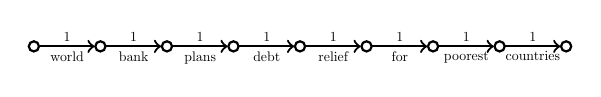
\begin{tikzpicture}[scale=0.65,
nod_s/.style = {scale=0.65, align=center, inner sep=2pt, text centered, circle, draw},
nod_m/.style = {nod_s, thick},
edge_ls/.style = {scale=0.5},
edge_lm/.style = {edge_ls, thick},
edge_ts/.style = {scale=0.5},
edge_tm/.style = {edge_ts},
]

%\newlength{\myx}
%\newlength{\myy}

\setlength{\myx}{1.3cm}
\setlength{\myy}{1.2cm}

\node(0) [nod_m] at (0\myx,0\myy) {};
\node(1) [nod_m] at (1\myx,0\myy) {};
\node(3) [nod_m] at (2\myx,0\myy) {};
\node(4) [nod_m] at (3\myx,0\myy) {};
\node(7) [nod_m] at (4\myx,0\myy) {};
\node(14) [nod_m] at (5\myx,0\myy) {};
\node(20) [nod_m] at (6\myx,0\myy) {};;
\node(27) [nod_m] at (7\myx,0\myy) {};
\node(35) [nod_m] at (8\myx,0\myy) {};

\draw[->,edge_lm] (0) to node [midway, sloped, below, edge_tm] {world\vphantom{pt}} node [midway, sloped, above, edge_tm] {1} (1);
\draw[->,edge_lm] (1) to node [midway, sloped, below, edge_tm] {bank\vphantom{pt}} node [midway, sloped, above, edge_tm] {1} (3);
\draw[->,edge_lm] (3) to node [midway, sloped, below, edge_tm] {plans\vphantom{pt}} node [midway, sloped, above, edge_tm] {1} (4);
\draw[->,edge_lm] (4) to node [midway, sloped, below, edge_tm] {debt\vphantom{pt}} node [midway, sloped, above, edge_tm] {1} (7);
\draw[->,edge_lm] (7) to node [midway, sloped, below, edge_tm] {relief\vphantom{pt}} node [midway, sloped, above, edge_tm] {1} (14);
\draw[->,edge_lm] (14) to node [midway, sloped, below, edge_tm] {for\vphantom{pt}} node [midway, sloped, above, edge_tm] {1} (20);
\draw[->,edge_lm] (20) to node [midway, sloped, below, edge_tm] {poorest\vphantom{pt}} node [midway, sloped, above, edge_tm] {1} (27);
\draw[->,edge_lm] (27) to node [midway, sloped, below, edge_tm] {countries\vphantom{pt}} node [midway, sloped, above, edge_tm] {1} (35);

\end{tikzpicture}
}
\caption{Illustration of rule application (1)}
\end{figure}

By using DFS to traverse the syntax tree, the program first finds out the pattern started from node ``VP'' with $2$ levels corresponds the left part of the first rule listed above. This indicates the rule is applicable at this position. According to the reordering rule, the order of the three constituents labeled with ``VBZ'', ``NP'' and ``PP'' should be changed to ``PP VBZ NP'' with probability $0.18$. Thus the words are reordered into ``for poorest countries plans debt relief'', and the new path with this probability is added to the word lattice.

\begin{figure}[H]
\centering
\subfigure{
\input{left2.tikz}
}
\subfigure{
\input{right2.tikz}
}
\caption{Illustration of rule application (2)}
\end{figure}

As the program keeps going, it turns out the second rule is applicable at another node labeled with ``NP'' with $2$ levels. Again the rule is applied with probability $0.17$ and the new path is added. It should be noted that there're numbers added to the two ``NN'' tags in the rule, in order to distinguish them for the reordering. The program uses index for the internal presentation of words, which doesn't cause any confusion.

\begin{figure}[H]
\centering
\subfigure{
\input{left3.tikz}
}
\subfigure{
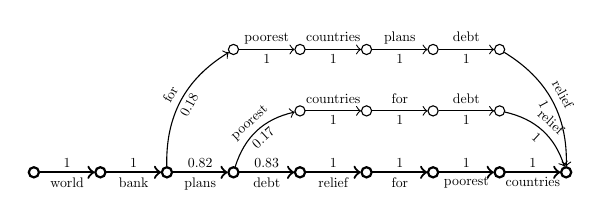
\begin{tikzpicture}[scale=0.65,
nod_s/.style = {scale=0.65, align=center, inner sep=2pt, text centered, circle, draw},
nod_m/.style = {nod_s, thick},
edge_ls/.style = {scale=0.5},
edge_lm/.style = {edge_ls, thick},
edge_ts/.style = {scale=0.5},
edge_tm/.style = {edge_ts},
]

%\newlength{\myx}
%\newlength{\myy}

\setlength{\myx}{1.3cm}
\setlength{\myy}{1.2cm}

\node(0) [nod_m] at (0\myx,0\myy) {};
\node(1) [nod_m] at (1\myx,0\myy) {};
\node(3) [nod_m] at (2\myx,0\myy) {};
\node(4) [nod_m] at (3\myx,0\myy) {};
\node(6) [nod_s] at (3\myx,2\myy) {};
\node(7) [nod_m] at (4\myx,0\myy) {};
\node(11) [nod_s] at (4\myx,1\myy) {};
\node(13) [nod_s] at (4\myx,2\myy) {};
\node(14) [nod_m] at (5\myx,0\myy) {};
\node(17) [nod_s] at (5\myx,1\myy) {};
\node(19) [nod_s] at (5\myx,2\myy) {};
\node(20) [nod_m] at (6\myx,0\myy) {};
\node(24) [nod_s] at (6\myx,1\myy) {};
\node(26) [nod_s] at (6\myx,2\myy) {};
\node(27) [nod_m] at (7\myx,0\myy) {};
\node(32) [nod_s] at (7\myx,1\myy) {};
\node(34) [nod_s] at (7\myx,2\myy) {};
\node(35) [nod_m] at (8\myx,0\myy) {};

\draw[->,edge_lm] (0) to node [midway, sloped, below, edge_tm] {world\vphantom{pt}} node [midway, sloped, above, edge_tm] {1} (1);
\draw[->,edge_lm] (1) to node [midway, sloped, below, edge_tm] {bank\vphantom{pt}} node [midway, sloped, above, edge_tm] {1} (3);
\draw[->,edge_lm] (3) to node [midway, sloped, below, edge_tm] {plans\vphantom{pt}} node [midway, sloped, above, edge_tm] {0.82} (4);
\draw[->,edge_ls] (3) to [bend left] node [midway, sloped, above, edge_ts] {for\vphantom{pt}} node [midway, sloped, below, edge_ts] {0.18} (6);
\draw[->,edge_lm] (4) to node [midway, sloped, below, edge_tm] {debt\vphantom{pt}} node [midway, sloped, above, edge_tm] {0.83} (7);
\draw[->,edge_ls] (4) to [bend left] node [midway, sloped, above, edge_ts] {poorest\vphantom{pt}} node [midway, sloped, below, edge_ts] {0.17} (11);
\draw[->,edge_ls] (6) to node [midway, sloped, above, edge_ts] {poorest\vphantom{pt}} node [midway, sloped, below, edge_tm] {1} (13);
\draw[->,edge_lm] (7) to node [midway, sloped, below, edge_tm] {relief\vphantom{pt}} node [midway, sloped, above, edge_tm] {1} (14);
\draw[->,edge_ls] (11) to node [midway, sloped, above, edge_ts] {countries\vphantom{pt}} node [midway, sloped, below, edge_tm] {1} (17);
\draw[->,edge_ls] (13) to node [midway, sloped, above, edge_ts] {countries\vphantom{pt}} node [midway, sloped, below, edge_tm] {1} (19);
\draw[->,edge_lm] (14) to node [midway, sloped, below, edge_tm] {for\vphantom{pt}} node [midway, sloped, above, edge_tm] {1} (20);
\draw[->,edge_ls] (17) to node [midway, sloped, above, edge_ts] {for\vphantom{pt}} node [midway, sloped, below, edge_tm] {1} (24);
\draw[->,edge_ls] (19) to node [midway, sloped, above, edge_ts] {plans\vphantom{pt}} node [midway, sloped, below, edge_tm] {1} (26);
\draw[->,edge_lm] (20) to node [midway, sloped, below, edge_tm] {poorest\vphantom{pt}} node [midway, sloped, above, edge_tm] {1} (27);
\draw[->,edge_ls] (24) to node [midway, sloped, above, edge_ts] {debt\vphantom{pt}} node [midway, sloped, below, edge_tm] {1} (32);
\draw[->,edge_ls] (26) to node [midway, sloped, above, edge_ts] {debt\vphantom{pt}} node [midway, sloped, below, edge_tm] {1} (34);
\draw[->,edge_lm] (27) to node [midway, sloped, below, edge_tm] {countries\vphantom{pt}} node [midway, sloped, above, edge_tm] {1} (35);
\draw[->,edge_ls] (32) to [bend left] node [midway, sloped, above,  edge_ts] {relief\vphantom{pt}} node [midway, sloped, below, edge_tm] {1} (35);
\draw[->,edge_ls] (34) to [bend left] node [midway, sloped, above,  edge_ts] {relief\vphantom{pt}} node [midway, sloped, below, edge_tm] {1} (35);

\end{tikzpicture}
}
\caption{Illustration of rule application (3)}
\end{figure}

\section{Summary}

advantages